\documentclass[11pt]{article}

% ACL style
\usepackage[preprint]{acl}

% Fonts
\usepackage{iftex}
\ifPDFTeX
  \usepackage[T5,T1]{fontenc}
  \usepackage[utf8]{inputenc}
  \usepackage{times}
  \usepackage{inconsolata}
\else
  \usepackage{fontspec}
  \setmainfont{Times New Roman}
  \setmonofont{Courier New}
\fi

% Packages
\usepackage{graphicx}
\usepackage{booktabs}
\usepackage{multirow}
\usepackage[normalem]{ulem}
\usepackage{amsmath}
\usepackage{amssymb}
\usepackage{url}
\usepackage{xurl}
\usepackage{float}
\usepackage{algorithm}
\usepackage{algpseudocode}

\graphicspath{{figures/}{../llm2seq/figures/}{llm2seq/figures/}}

\newlength{\demoimageboxheight}
\setlength{\demoimageboxheight}{0.32\textheight}
\newcommand{\framedemoimage}[1]{%
  \begingroup
  \setlength{\fboxsep}{2pt}%
  \setlength{\fboxrule}{0.4pt}%
  \fbox{%
    \begin{minipage}[c][\demoimageboxheight][c]{\dimexpr\linewidth-2\fboxsep-2\fboxrule\relax}
    \centering
    \includegraphics[
      width=\linewidth,
      height=\dimexpr\demoimageboxheight-4pt\relax,
      keepaspectratio
    ]{#1}%
    \end{minipage}%
  }%
  \endgroup
}

\makeatletter
\setlength{\@dblfptop}{0pt}
\makeatother

\title{LLM2Seq: Repurposing LLM Encoders for Encoder-Decoder Summarization with Self-Distilled Multi-Token Prediction}

\author{
  Giang-Bien Kieu$^1$ \quad Xuan-Dung Doan$^2$ \\
  $^1$Hanoi University of Science and Technology, HUST, Vietnam \\
  $^2$Viettel Artificial Intelligence Center, Viettel Group, Vietnam \\
  \texttt{bienkieugiang@gmail.com} \quad \texttt{dungdx4@viettel.com.vn}
}

\begin{document}
\maketitle

\begin{abstract}
Abstractive summarization requires modeling a source document and generating a concise target sequence, making encoder-decoder architectures a natural fit.
Modern Large Language Model (LLM) checkpoints provide strong representations, but many do not expose a direct encoder-decoder interface for summarization.
This report presents LLM2Seq, an encoder-decoder summarizer that repurposes pretrained LLM-based encoders to represent source documents.
A gated residual adapter converts their hidden states into decoder-readable cross-attention memory, and a lightweight Transformer decoder generates the summary.
On WikiLingua, we further study inference acceleration with self-distilled Multi-Token Prediction (MTP): after summarizer training, MTP heads learn from the frozen decoder, draft future tokens, and are verified by the main decoder during inference.

We evaluate LLM2Seq on Vietnamese WikiLingua and add a Vietnamese LR-Sum evaluation.
The results show that LLM-based encoders can provide useful cross-attention memory for summarization.
The WikiLingua MTP results further show that decoding acceleration should be evaluated by real throughput, not only by accepted-token statistics.
\end{abstract}

\noindent\textbf{Keywords:} abstractive summarization; encoder-decoder models; LLM-based encoders; adapters; multi-token prediction; Vietnamese WikiLingua; LR-Sum

\section{Introduction}
\label{sec:introduction}

\subsection{Motivation}

Abstractive summarization is a sequence-to-sequence task.
The model reads a source document and writes a shorter summary \citep{sutskever2014sequence,bahdanau2015neural,vaswani2017attention}.
Encoder-decoder architectures naturally match this setting by separating source understanding from target generation.
Many modern LLMs are decoder-only models \citep{brown2020language,dubey2024llama3,yang2024qwen2}.
Although they are strong generators, they encode the source and target within a single causal stream.
This makes the source-summary boundary less clear.

\subsection{Problem Statement}

We ask whether pretrained LLM-based encoders can be reused inside an encoder-decoder summarizer.
We study Vietnamese WikiLingua \citep{ladhak2020wikilingua} and add a follow-up evaluation on Vietnamese LR-Sum \citep{palen-michel-lignos-2023-lr}.
The goal is to keep strong source representations, expose them through cross-attention, and speed up decoding when possible.

\subsection{Gap with Existing Work}

T5, BART, and mT5 are strong encoder-decoder models \citep{raffel2020t5,lewis2020bart,xue2021mt5}.
They do not directly reuse newer LLM checkpoints.
Recent work shows that decoder-only LLMs can become useful encoders \citep{behnamghader2024llm2vec,luo2025lamate}.
For summarization, however, these representations still need a stable bridge into decoder cross-attention.

Context compression methods such as LCLMs compress long prompts into short latent sequences \citep{li2026contextcompression}.
This helps general long-context inference.
Source-grounded summarization places different pressure on the representation, because summaries often need names, numbers, steps, and local details.
If the source is compressed too early, the decoder may lose these details.
LLM2Seq keeps token-level memory instead.

\subsection{Contributions}

We propose \textbf{LLM2Seq}.
It is an encoder-decoder summarizer built from repurposed LLM-based encoders.
\begin{itemize}
    \item We adapt LLM-based encoders for Vietnamese abstractive summarization on WikiLingua and LR-Sum.
    \item We introduce a gated residual memory adapter that converts LLM hidden states into decoder-readable cross-attention memory.
    \item On WikiLingua, we train self-distilled MTP heads after the summarizer is trained \citep{gloeckle2024mtp,zhao2026mtpdistill}.
    \item On WikiLingua, we show that MTP should be evaluated by real throughput rather than accepted-token statistics alone.
\end{itemize}

\section{Background and Related Work}
\label{sec:related}

\subsection{Encoder-Decoder Summarization}

Encoder-decoder models separate reading and writing.
The decoder attends to encoder states while generating the summary.
This interface comes from attention-based sequence-to-sequence models and Transformers \citep{sutskever2014sequence,bahdanau2015neural,vaswani2017attention}.
T5, BART, and mT5 show that it works well for summarization \citep{raffel2020t5,lewis2020bart,xue2021mt5}.

\subsection{Decoder-only LLMs as Encoders}

Decoder-only LLMs are trained for next-token prediction.
Their causal mask is good for generation, but less direct for source encoding.
LLM2Vec shows that decoder-only LLMs can be converted into text encoders \citep{behnamghader2024llm2vec}.
LaMaTE uses LLM encoders for machine translation \citep{luo2025lamate}.
T5Gemma builds encoder-decoder models from modern decoder-only components \citep{zhang2025t5gemma2}.
LLM2Seq follows this direction for summarization.

\subsection{Context Compression and LCLM}

LCLMs compress long contexts into short latent sequences for general long-context inference \citep{li2026contextcompression}.
They optimize compression ratio, memory, and long-context accuracy.
LLM2Seq has a different goal.
It keeps token-level memory because summaries often need local evidence.

\subsection{Efficient Decoding and MTP}

Autoregressive decoding emits one token per step.
Speculative decoding drafts and verifies tokens \citep{leviathan2023speculative}.
Blockwise decoding and Medusa also try to emit more than one token per step \citep{stern2018blockwise,cai2024medusa}.
MTP trains heads to predict future tokens \citep{gloeckle2024mtp}.
MTP-D improves these heads with self-distillation \citep{zhao2026mtpdistill,hinton2015distilling}.

\subsection{Positioning of LLM2Seq}

LLM2Seq is not a context compressor.
It is also not a pure prompting method.
It studies whether LLM-derived source states can become useful decoder memory for summarization.
On WikiLingua, it also tests whether verified MTP gives real speedup \citep{gloeckle2024mtp,zhao2026mtpdistill}.
Table~\ref{tab:lclm-position} compares it with LCLM-style compression \citep{li2026contextcompression}.

\begin{table*}[t]
\centering
\small
\begin{tabular}{p{0.19\textwidth}p{0.36\textwidth}p{0.36\textwidth}}
\toprule
Aspect & LCLM / End-to-End Context Compression & LLM2Seq \\
\midrule
Main goal & Compress long context for general inference & Vietnamese abstractive summarization \\
Source representation & Short latent compressed sequence & Token-level cross-attention memory \\
Compression ratio & Explicit optimization target & Not the main objective \\
Output setting & General long-context inference & Encoder-decoder summary generation \\
Speed mechanism & Shorter context and reduced memory & Verified MTP decoding \\
Risk & Information loss from compression & More memory and cross-attention cost \\
Best use case & Long redundant context & Source-grounded summarization \\
\bottomrule
\end{tabular}
\caption{Conceptual comparison with LCLM-style context compression. This is not an empirical LCLM baseline.}
\label{tab:lclm-position}
\end{table*}

\section{LLM2Seq Method}
\label{sec:method}

\begin{figure*}[t]
\centering
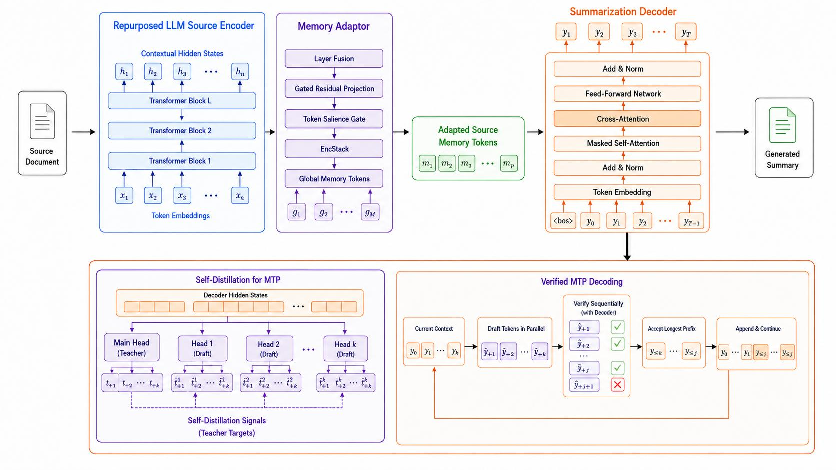
\includegraphics[width=0.98\textwidth]{figures/architecture.pdf}
\caption{Overall LLM2Seq architecture with the source encoder, memory adapter, decoder, and MTP modules.}
\label{fig:architecture}
\end{figure*}

\subsection{Problem Formulation}

Let $x=(x_1,\ldots,x_m)$ be the source document and $y=(y_1,\ldots,y_n)$ be the target summary.
Let $a^x_i\in\{0,1\}$ and $a^y_t\in\{0,1\}$ be the source and target masks.
The model estimates:
\begin{equation}
p(y|x)=\prod_{t=1}^{n}p(y_t \mid y_{<t},x).
\end{equation}
LLM2Seq makes the conditioning path explicit.
The source encoder builds token states:
\begin{equation}
H=E_{\theta}(x), \qquad H \in \mathbb{R}^{m \times d_e}.
\end{equation}
The adapter maps them into decoder memory:
\begin{equation}
M=A_{\phi}(H), \qquad M \in \mathbb{R}^{(m+g) \times d_d},
\end{equation}
where $g$ is the number of learned global memory tokens.
This memory $M$ is the source-memory block shown in Figure~\ref{fig:architecture}.
The decoder then generates:
\begin{equation}
p(y|x)=\prod_{t=1}^{n}p_{\psi}(y_t \mid y_{<t},M).
\end{equation}
Training uses teacher forcing.
With non-padding target positions $\Omega=\{t:a^y_t=1\}$, the summarization loss is:
\begin{equation}
\mathcal{L}_{sum}
=-\frac{1}{|\Omega|}\sum_{t\in\Omega}
\log p_{\psi}(y_t\mid y_{<t},M).
\end{equation}
This form is the core design choice.
The encoder focuses on source understanding, the decoder handles target generation, and the adapter controls how source evidence is exposed to cross-attention.

\subsection{Overall Architecture}

Figure~\ref{fig:architecture} shows the full system.
LLM2Seq has three main parts.
First, it uses a pretrained LLM-based encoder on the source side.
We instantiate it with either an LLM2Vec-derived Llama encoder or a Qwen embedding encoder \citep{behnamghader2024llm2vec,zhang2025qwen3embedding}.
Second, a gated residual memory adapter reshapes the encoder states into decoder memory.
In Figure~\ref{fig:architecture}, \textit{memory adapter} denotes the complete bridge from LLM hidden states to decoder-readable cross-attention memory, including learned global tokens and adapted token-level source states.
Third, a lightweight Transformer decoder generates the summary with masked self-attention and cross-attention \citep{vaswani2017attention}.
After the summarizer is trained, an MTP module is attached for acceleration.
The MTP module is trained separately and verified by the main decoder during inference.

\subsection{Repurposed LLM-Based Encoder}

We use two source-side LLM encoders.
The Llama variant uses an LLM2Vec Sheared-LLaMA checkpoint \citep{behnamghader2024llm2vec}.
The Qwen variant uses Qwen3-Embedding-0.6B \citep{zhang2025qwen3embedding}.
This distinction defines the scope of the claim: LLM2Seq studies reusable LLM-based encoders, not only pure decoder-only checkpoints.
For a source sequence $x$, the encoder returns token-level hidden states:
\begin{equation}
H^{(\ell)}=F^{(\ell)}_{\theta}(x,a^x),
\qquad
H^{(\ell)}\in\mathbb{R}^{m\times d_e}.
\end{equation}
Unlike sentence embedding use cases, LLM2Seq keeps the full sequence of token states.
This is needed because the decoder must attend to local source evidence.
The encoder also returns a set of selected layers:
\begin{equation}
\mathcal{H}_S=\{H^{(l_1)},H^{(l_2)},\ldots,H^{(l_s)}\}.
\end{equation}
In our setting, the selected layers are $[-1,-4,-8,-12]$.
Full fine-tuning is expensive.
Phase 2 therefore applies LoRA to the encoder \citep{hu2022lora}.
For a frozen encoder weight matrix $W$, LoRA learns a low-rank update:
\begin{equation}
W'=W+\frac{\alpha}{r}BA,
\end{equation}
where $A\in\mathbb{R}^{r\times d_{in}}$ and
$B\in\mathbb{R}^{d_{out}\times r}$.
Only the low-rank matrices are updated for the encoder.
This adapts the source representation to Vietnamese summarization while keeping training practical.

\subsection{Gated Residual Memory Adapter}

The adapter bridges the LLM encoder and the decoder.
It resolves a representation mismatch: encoder states live in the LLM space, whereas the decoder expects memory in its own hidden space.
At the same time, it preserves token-level evidence because summaries often depend on details in the source.
The contribution is the organization of familiar mechanisms into a source-memory bridge for summarization: layer mixing, gated updates, feature modulation, Transformer refinement, and learned memory tokens.

First, token-wise layer fusion combines selected encoder layers.
This is inspired by learned layer mixing in contextual representation models such as ELMo \citep{peters2018elmo}.
The adaptation in LLM2Seq is token-wise rather than document-global: each source token can choose a different mixture over selected LLM layers.
For token position $i$ and selected layer $j$, a score is computed by:
\begin{equation}
e_{ij}=w_f^\top H^{(l_j)}_i.
\end{equation}
The layer mixture is:
\begin{equation}
\alpha_{ij}
=\frac{\exp(e_{ij})}{\sum_{r=1}^{s}\exp(e_{ir})},
\qquad
\bar{H}_i=\sum_{j=1}^{s}\alpha_{ij}H^{(l_j)}_i.
\end{equation}
This lets different tokens use different depths of the LLM.
Lexical cues and semantic cues do not always appear at the same layer.

The fused states are then projected into decoder space.
We use a gated residual projection for this step.
Gated residual mechanisms are widely used to modulate feature updates.
Examples include Highway Networks and gated linear units \citep{srivastava2015highway,dauphin2017glu}.
Here, the gate is used for the specific interface between a frozen or lightly adapted LLM encoder and a smaller cross-attentive decoder.
The implemented gated residual projection first normalizes the fused state:
\begin{equation}
\hat{H}=\operatorname{LN}(\bar{H}).
\end{equation}
It builds a base path, a gate, and an update:
\begin{equation}
P=W_p\hat{H}+b_p,
\qquad
G=\sigma(W_g\hat{H}+b_g),
\end{equation}
\begin{equation}
U=W_2\operatorname{GELU}(W_1\operatorname{LN}(P)+b_1)+b_2.
\end{equation}
The adapted token state is:
\begin{equation}
R=P+G\odot U.
\end{equation}
The base path $P$ maps the encoder states into the decoder dimension.
The update block $U$ adds task-specific changes.
The gate $G$ controls how much of this update is used.
This residual form keeps the original source information easier to preserve while still allowing the adapter to add summarization-specific corrections.

A token salience gate then estimates which source positions should be emphasized.
This gate is inspired by feature recalibration and feature-wise conditioning mechanisms such as Squeeze-and-Excitation and FiLM \citep{hu2018squeeze,perez2018film}.
LLM2Seq adapts this idea to token-level source memory by rescaling representations before decoder cross-attention.
\begin{equation}
S=\sigma(W_{s2}\operatorname{GELU}(W_{s1}\operatorname{LN}(R)+b_{s1})+b_{s2}).
\end{equation}
Our Token Salience Gate differs from token pruning and token selection methods.
Instead of suppressing or discarding low-salience tokens, it performs continuous feature rescaling:
\begin{equation}
R'_i=(0.5+S_i)R_i,
\end{equation}
ensuring every token contributes while allowing salient representations to be emphasized.
Padding positions have $S_i=0$.
Thus padded memory cannot become salient.

An EncStack refines the memory with $L_a=4$ pre-norm Transformer encoder layers \citep{vaswani2017attention}.
This part is a direct application of standard Transformer encoder refinement.
In LLM2Seq, it is placed after the projection and salience gate so that adapted source tokens can interact before they are read by the decoder.
\begin{equation}
\bar{R}^{(0)}=R',
\end{equation}
\begin{equation}
Q^{(u)}=\bar{R}^{(u-1)}
+\operatorname{SelfAttn}(\operatorname{LN}(\bar{R}^{(u-1)}),a^x),
\end{equation}
\begin{equation}
\bar{R}^{(u)}=Q^{(u)}
+\operatorname{FFN}(\operatorname{LN}(Q^{(u)})).
\end{equation}
Let $\tilde{R}=\bar{R}^{(L_a)}$.
The final memory concatenates learned global memory tokens $G_m$ with the refined token memory.
Learned global tokens are inspired by prefix tuning and prompt tuning \citep{li2021prefix,lester2021prompt}.
In contrast to prompts prepended to the decoder input, these tokens act as decoder-visible source-memory slots trained for summarization.
\begin{equation}
M=[G_m;\,\tilde{R}].
\end{equation}
The corresponding memory mask is:
\begin{equation}
a^M=[\mathbf{1}_g;\,a^x].
\end{equation}
The global tokens give the decoder a small document-level workspace.
The token memory gives the decoder direct access to local evidence.
Together, this concatenated sequence $M$ forms the \textit{adapted source memory tokens}.
In the rest of this report, \textit{adapted source memory} refers to this sequence $M=[G_m;\tilde{R}]$.
It contains global memory tokens followed by adapted token-level source states.
It provides the decoder with both document-level context and fine-grained local details in a unified representation space.

\subsection{Lightweight Cross-Attentive Decoder}

The decoder is an 8-layer Transformer decoder \citep{vaswani2017attention}.
It uses causal self-attention, cross-attention to $M$, RoPE, RMSNorm, and SwiGLU \citep{su2021roformer}.
At step $t$, it reads $y_{<t}$ and the adapted source memory.
The next-token distribution is:
\begin{equation}
\begin{aligned}
o_t&=E^\top\operatorname{RMSNorm}(Y^{(L_d)}_t),\\
p_{\psi}(y_t\mid y_{<t},M)&=\operatorname{softmax}(o_t).
\end{aligned}
\end{equation}
The decoder is intentionally smaller than the encoder.
This keeps generation cheaper while still allowing the encoder to carry strong source representations.

\subsection{Self-Distilled MTP}

After Phase 2, the main summarizer is frozen.
Phase 3 adds $K=4$ cascaded MTP heads \citep{gloeckle2024mtp,zhao2026mtpdistill,deepseekai2024deepseekv3}.
The heads predict future tokens beyond the next token.
The loss follows MTP-D style self-distillation.
The frozen main head acts as the teacher \citep{zhao2026mtpdistill,deepseekai2024deepseekv3}.
LLM2Seq uses this idea after summarizer training.
The encoder, adapter, decoder, and main LM head are frozen.
Only the MTP heads are updated.
This makes MTP a post-hoc speed module, not a joint pre-training objective.
Let $h_t^{(0)}=Y^{(L_d)}_t$ be the frozen decoder state at target position $t$.
The main head predicts:
\begin{equation}
p_t^{(0)}=\operatorname{softmax}(E^\top h_t^{(0)}).
\end{equation}
Each MTP depth $k$ predicts $y_{t+k}$:
\begin{equation}
p_t^{(k)}=\operatorname{softmax}(E^\top h_t^{(k)}),
\qquad k=1,\ldots,K.
\end{equation}
Let $\Omega_k=\{t:a^y_{t+k}=1\}$ denote positions whose $k$-step future target is valid.
The hard-label loss trains the heads on gold future tokens:
\begin{equation}
\mathcal{L}_{CE}
=-\frac{1}{\sum_{k=1}^{K}w_k}
\sum_{k=1}^{K}w_k
\frac{1}{|\Omega_k|}
\sum_{t\in\Omega_k}\log p_t^{(k)}(y_{t+k}).
\end{equation}
The KL loss makes each MTP head follow the frozen main head at the same future position \citep{hinton2015distilling}.
Let $q_{t,k}$ denote the teacher distribution from the frozen main head and $s_{t,k}$ denote the student distribution from the $k$-th MTP head, both restricted to the top-$J$ teacher logits.
The KL term is:
\begin{equation}
\mathcal{L}_{KL}
=\frac{\tau^2}{\sum_{k=1}^{K}w_k}
\sum_{k=1}^{K}w_k
\frac{1}{|\Omega_k|}
\sum_{t\in\Omega_k}\operatorname{KL}(q_{t,k}\,\|\,s_{t,k}).
\end{equation}
The final Phase 3 loss is:
\begin{equation}
\mathcal{L}_{MTP}
=\lambda_{CE}\mathcal{L}_{CE}
+\gamma(u)\lambda_{KL}\mathcal{L}_{KL},
\end{equation}
Here, $\gamma(u)$ gradually ramps in the KL term during training.
Only the MTP heads are updated in this phase.

\subsection{Verified MTP Decoding Algorithm}

At inference time, the MTP heads draft future tokens.
The main decoder verifies them.
This follows the draft-and-verify idea in speculative decoding and MTP-style decoding \citep{leviathan2023speculative,gloeckle2024mtp,zhao2026mtpdistill}.
Let $g(\pi)$ be the constrained greedy main-head token for prefix $\pi$.
It includes the same repetition penalty, minimum length rule, and no-repeat trigram constraint as standard decoding.
For a current prefix $\pi$, the main decoder first predicts $c_0=g(\pi)$.
The MTP module then drafts future tokens:
\begin{equation}
c_k=\operatorname*{arg\,max}_{v}
p^{(k)}(v\mid \pi,c_{<k}),
k=1,\ldots,K.
\end{equation}
The candidate block is $c=(c_0,c_1,\ldots,c_K)$.
The verifier runs the frozen decoder on this block.
It accepts the longest draft prefix that matches the main decoder.
The first mismatch is corrected by the verifier token.
Algorithm~\ref{alg:mtp_decoding} gives the procedure.

\begin{algorithm}[H]
\caption{Verified MTP Draft-and-Check Decoding}
\label{alg:mtp_decoding}
\begin{algorithmic}[1]
\State Encode the source once and cache cross-attention keys and values.
\Repeat
    \State Predict the main token $c_0$ from the current prefix.
    \State Draft $K$ future tokens with the cascaded MTP heads.
    \State Verify the candidate block with the frozen main decoder.
    \State Accept the longest draft prefix that matches the verifier.
    \State Emit the accepted prefix and the verifier correction token.
    \State Slice the decoder cache to the verified prefix.
\Until{the end token or the maximum length is reached}
\end{algorithmic}
\end{algorithm}
If step $s$ emits $e_s$ tokens, the average emitted tokens per step is:
\begin{equation}
\bar{e}=\frac{\sum_s e_s}{T},
\end{equation}
where $T$ is the number of verification steps.
A high $\bar{e}$ reduces the number of steps.
It does not guarantee higher throughput because verification also costs time.

\subsection{Training Procedure}

LLM2Seq uses three phases.
Phase 1 freezes the encoder and trains the adapter, decoder, global memory tokens, and LM head with $\mathcal{L}_{sum}$.
Phase 2 adds LoRA to the encoder and continues optimizing the summarization loss \citep{hu2022lora}.
Phase 3 freezes the main summarizer and trains only the MTP module with $\mathcal{L}_{MTP}$.
This ordering matters.
The summarizer is built first.
The speed module is trained after that.
Thus Phase 3 is a decoupled, post-hoc use of MTP for inference speed.
It is not the joint MTP pre-training objective from the original MTP papers \citep{gloeckle2024mtp,zhao2026mtpdistill,deepseekai2024deepseekv3}.

\subsection{Complexity and Inference Cost}

The encoder runs once per source document.
The autoregressive decoder then runs once per generated token.
Let $C_{\mathrm{AR}}$ be the average cost of one autoregressive decoding step.
If a summary has $n$ generated tokens, the decoding cost is roughly:
\begin{equation}
C_{\mathrm{decode}}^{AR}\approx nC_{\mathrm{AR}}.
\end{equation}
Verified MTP emits $\bar{e}$ tokens per step on average, but each step has extra draft and verification cost $C_{\mathrm{ver}}$:
\begin{equation}
C_{\mathrm{decode}}^{MTP}
\approx \frac{n}{\bar{e}}(C_{\mathrm{AR}}+C_{\mathrm{ver}}).
\end{equation}
MTP is faster only when:
\begin{equation}
\bar{e} > 1+\frac{C_{\mathrm{ver}}}{C_{\mathrm{AR}}}.
\end{equation}
The condition explains why accepted tokens and real throughput can disagree.
The system must save more decoder steps than it adds in verification overhead.

\section{Experimental Setup}
\label{sec:setup}
\suppressfloats[t]

\subsection{Dataset and Preprocessing}

We evaluate on the Vietnamese subset of WikiLingua, a multilingual abstractive summarization dataset extracted from WikiHow articles \citep{ladhak2020wikilingua}.
Both source articles and summaries are Vietnamese.
The original WikiLingua release reports 19,600 Vietnamese article-summary pairs.
Our local split contains 19,581 raw records.
Preprocessing removes one test example with an empty source, leaving 19,580 examples.
Table~\ref{tab:data-split} summarizes the split.

We also evaluate on the Vietnamese split of LR-Sum \citep{palen-michel-lignos-2023-lr}.
LR-Sum is a multilingual news summarization dataset for less-resourced languages, with human-written summaries from Voice of America newswire.
The Vietnamese split contains 14,595 examples in our processed copy, as shown in Table~\ref{tab:lrsum-data-split}.
For LR-Sum, we use the article text as the source and the summary field as the target.

\begin{table}[htbp]
\centering
\small
\begin{tabular}{lrr}
\toprule
Split & Raw & Used \\
\midrule
Train & 13,999 & 13,999 \\
Validation & 1,680 & 1,680 \\
Test & 3,902 & 3,901 \\
\midrule
Total & 19,581 & 19,580 \\
\bottomrule
\end{tabular}
\caption{Vietnamese WikiLingua data split.}
\label{tab:data-split}
\end{table}

\begin{table}[htbp]
\centering
\small
\begin{tabular}{lrr}
\toprule
Split & Raw & Used \\
\midrule
Train & 11,676 & 11,676 \\
Validation & 1,459 & 1,459 \\
Test & 1,460 & 1,460 \\
\midrule
Total & 14,595 & 14,595 \\
\bottomrule
\end{tabular}
\caption{Vietnamese LR-Sum data split.}
\label{tab:lrsum-data-split}
\end{table}

\subsection{Compared Systems and Baselines}

We compare three systems.
\textbf{LLM2Seq-Llama} uses the LLM2Vec-Sheared-LLaMA encoder \citep{behnamghader2024llm2vec}.
\textbf{LLM2Seq-Qwen} uses the Qwen3-Embedding-0.6B encoder \citep{zhang2025qwen3embedding}.
Both use the same adapter and lightweight decoder design.
\textbf{T5Gemma} is a T5Gemma-2-1B-1B LoRA baseline \citep{zhang2025t5gemma2,hu2022lora}.

\subsection{Implementation Details}

The WikiLingua source length is up to 3,072 tokens and the target length is up to 384 tokens during training.
For LR-Sum, the source length remains 3,072 tokens and the target length is 256 tokens.
Generation uses at most 256 new tokens.
All reported systems use greedy decoding and no-repeat trigram blocking.
LLM2Seq uses bf16/tf32 training.
Both LLM2Seq variants adapt the encoder with LoRA \citep{hu2022lora}.
For the WikiLingua experiments, the MTP module uses four heads and is trained after the main summarizer is frozen.
We use AdamW with betas $(0.9,0.95)$ and $\epsilon=10^{-8}$, a linear warmup, cosine decay, and gradient clipping at 1.0.
For WikiLingua, Phase 1 trains the adapter and decoder for 6 epochs.
It uses batch size 24, gradient accumulation 2, learning rate $2\cdot10^{-4}$, warmup ratio 0.03, and weight decay 0.01.
Phase 2 adapts the encoder with LoRA.
For WikiLingua, Phase 2 runs for 6 epochs.
It uses batch size 16, gradient accumulation 2, encoder learning rate $5\cdot10^{-4}$, decoder and adapter learning rate $5\cdot10^{-5}$, and weight decay 0.05.
Both WikiLingua LLM2Seq runs also use gradual unfreezing.
On WikiLingua, Phase 3 freezes the encoder, adapter, and decoder.
It trains only the MTP heads for 6 epochs.
It uses batch size 20, gradient accumulation 4, learning rate $5\cdot10^{-4}$, warmup ratio 0.05, and weight decay 0.01.
For LR-Sum, the LLM2Seq runs cover Phase 1--2 quality evaluation only.
They do not include Phase 3 MTP.
The LR-Sum Llama runs use 3 epochs for Phase 1 and 3 epochs for Phase 2; LR-Sum Qwen uses 3 epochs for Phase 1 and 6 epochs for Phase 2.
Checkpoints are selected by validation loss.
For generation, all WikiLingua models use a minimum of 32 new tokens and repetition penalty 1.15.
For LR-Sum, the available runs use a minimum of 32 new tokens and repetition penalty 1.05.
The WikiLingua T5Gemma baseline is trained for 6 epochs with LoRA.
It uses batch size 16, gradient accumulation 2, learning rate $2\cdot10^{-4}$, warmup ratio 0.03, weight decay 0.01, cosine schedule, and fused AdamW.
The LR-Sum T5Gemma run is trained for 3 epochs.
Appendix~\ref{app:hparams} summarizes the training and decoding configuration.

\subsection{Evaluation Metrics}

We report ROUGE \citep{lin2004rouge}, BERTScore \citep{zhang2020bertscore}, length statistics, and speed.
ROUGE-1 and ROUGE-2 measure unigram and bigram overlap.
ROUGE-L measures longest common subsequence overlap.
We report macro-averaged F1 for all ROUGE scores.
For Vietnamese text, ROUGE is computed with the HeterSumGraph protocol using
\texttt{rouge==1.0.0} and \texttt{Rouge().get\_scores(..., avg=True)}.
Both predictions and references are normalized to Unicode NFC and lowercase;
the stored whitespace and punctuation tokenization is otherwise preserved.
Length statistics use whitespace-separated tokens from \texttt{text.split()}, which we call words for readability.
We do not apply Vietnamese word segmentation such as VnCoreNLP or underthesea.
This choice is important because Vietnamese word segmentation can change overlap scores.
For length, we report mean predicted words and too-long rate.
The too-long rate is the percentage of predictions whose word count is more than 1.5 times the reference word count.
BERTScore is computed with \texttt{bert-base-multilingual-cased}.
It matches generated and reference tokens by contextual embedding similarity.
We report precision, recall, and F1 as percentages.
BERTScore is more semantic than ROUGE, but it is not a factuality metric.
All BERTScore values reported in the main result tables use \texttt{bert-base-multilingual-cased}.
For speed, we report generated tokens per second and mean latency.
We compare speed only when the batch setting is the same.
When comparing AR and MTP speed on WikiLingua, we use paired comparison logs under the same model and batch setting.

\subsection{Research Questions}

We evaluate LLM2Seq with three questions.
They cover summarization quality, encoder configuration, and decoding speed.
\begin{itemize}
    \item \textbf{RQ1}: Can pretrained LLM-based encoders be reused inside an encoder-decoder summarizer?
    \item \textbf{RQ2}: On WikiLingua, how much do the LLM2Seq encoder configurations affect quality, length, and speed?
    \item \textbf{RQ3}: On WikiLingua, does verified MTP improve real throughput, or does it only reduce decoding steps?
\end{itemize}

\section{Results and Analysis}
\label{sec:results}

\subsection{RQ1: Viability of LLM-Based Encoders}

Table~\ref{tab:main-results} reports WikiLingua and LR-Sum test results.
On WikiLingua, the Qwen-based LLM2Seq system achieves 24.14 ROUGE-1, 8.04 ROUGE-2, 24.55 ROUGE-L, and 73.42 BERTScore F1.
The WikiLingua result shows that a pretrained LLM-based encoder can provide useful cross-attention memory for an encoder-decoder summarizer.
On WikiLingua, the Llama-based system also produces valid summaries.
Its ROUGE scores are lower, and its outputs are much shorter.
These differences indicate that encoder configuration has a substantial effect on output length and ROUGE.

On WikiLingua, LLM2Seq-Qwen is better than the Llama configuration, but T5Gemma is higher on all three ROUGE metrics.
The result supports the LLM2Seq design, but it does not show that LLM2Seq outperforms T5Gemma.
It also depends on the encoder choice and output length.

\begin{table*}[t]
\centering
\small
\setlength{\tabcolsep}{3pt}
\begin{tabular}{llrrrrrrrr}
\toprule
Dataset & Model & R-1 & R-2 & R-L & BERT-P & BERT-R & BERT-F1 & Avg. Words & Too Long (\%) \\
\midrule
\multirow{3}{*}{WikiLingua} & LLM2Seq-Llama & 17.28 & 4.70 & 18.71 & \textbf{74.08} & 72.11 & 73.02 & 29.10 & 5.46 \\
 & LLM2Seq-Qwen & 24.14 & 8.04 & 24.55 & 72.87 & 74.11 & 73.42 & 58.31 & 35.79 \\
 & T5Gemma & \textbf{33.10} & \textbf{13.76} & \textbf{31.64} & 71.99 & \textbf{78.40} & \textbf{74.98} & 90.89 & 68.03 \\
\midrule
\multirow{3}{*}{LR-Sum} & LLM2Seq-Llama & 12.83 & 2.74 & 10.16 & 70.74 & 69.26 & 69.98 & 26.78 & 4.18 \\
 & LLM2Seq-Qwen & 18.71 & 5.84 & 15.60 & 72.24 & 71.04 & 71.62 & 29.50 & 6.92 \\
 & T5Gemma & \textbf{30.09} & \textbf{18.42} & \textbf{27.31} & \textbf{74.13} & \textbf{75.24} & \textbf{74.65} & 33.73 & 14.18 \\
\bottomrule
\end{tabular}
\caption{Test results on WikiLingua and Vietnamese LR-Sum.
Scores are percentages.
BERTScore uses \texttt{bert-base-multilingual-cased} without baseline rescaling.
\textbf{Avg. Words} is mean output length.
\textbf{Too Long} is the percentage of predictions with more than 1.5x the reference word count.}
\label{tab:main-results}
\end{table*}

On LR-Sum, LLM2Seq-Qwen improves over LLM2Seq-Llama.
The gain is clearest on ROUGE-2 and BERTScore F1.
Its average output length is also close to the reference length.
T5Gemma still achieves substantially higher ROUGE-1, ROUGE-2, and ROUGE-L scores.
The LR-Sum LLM2Seq outputs are fluent, but they can choose wrong entities or events.
Such errors lower n-gram overlap with the reference.

\subsection{RQ2: Effect of Encoder Configuration on WikiLingua}

On WikiLingua, the two LLM2Seq variants behave differently.
LLM2Seq-Llama under-generates.
Its average output length is 29.10 words, far below the 51.86-word reference average.
LLM2Seq-Qwen generates longer summaries.
Its average output length is 58.31 words, which is closer to the reference.
The length difference partly explains the large ROUGE gap between the two LLM2Seq variants.

The WikiLingua comparison should be read as a controlled configuration-level comparison rather than a pure encoder-only ablation.
Both variants use the same overall LLM2Seq architecture, adapter design, decoder design, and decoding constraints.
However, changing the source-side encoder also changes the tokenizer, vocabulary, and representation space.

Table~\ref{tab:speed} shows WikiLingua autoregressive decoding speed.
LLM2Seq-Llama is faster than LLM2Seq-Qwen: 114.74 tokens/s versus 95.87 tokens/s.
A likely explanation is the decoder-side vocabulary size.
Because the decoder uses a tied input/output embedding matrix, the final LM head depends on the tokenizer vocabulary.
The larger Qwen vocabulary can make each decoding step more expensive.
At the same time, Qwen gives better summarization quality.
The result suggests a quality-speed trade-off on WikiLingua: Qwen improves quality and length control, while Llama is faster but under-generates.

\begin{table}[t]
\centering
\small
\begin{tabular}{lrr}
\toprule
Model & tok/s & Mean latency \\
\midrule
LLM2Seq-Llama & 114.74 & 0.697s \\
LLM2Seq-Qwen & 95.87 & 0.779s \\
\bottomrule
\end{tabular}
\caption{Autoregressive decoding speed for LLM2Seq variants on WikiLingua under the same batch setting.}
\label{tab:speed}
\end{table}

\subsection{RQ3: Verified MTP Throughput on WikiLingua}

Table~\ref{tab:mtp-results} compares autoregressive decoding and verified MTP for the Qwen-based system on WikiLingua.
Verified MTP increases the emitted tokens per decoding step from 1.00 to 2.30 and improves throughput from 95.87 tokens/s to 111.71 tokens/s.
The measured speedup is 1.17x, with mean latency decreasing from 0.779s to 0.662s.

\begin{table*}[t]
\centering
\small
\begin{tabular}{llrrrrrrrrr}
\toprule
Model & Mode & tok/s & Spd. & Lat. & Emit & Draft & R-1 & R-2 & R-L & BERT-F1 \\
\midrule
Llama & AR & 114.74 & 1.00x & 0.697 & 1.00 & 0.00 & 17.28 & 4.70 & 18.71 & 73.02 \\
Qwen & AR & 95.87 & 1.00x & 0.779 & 1.00 & 0.00 & 24.14 & 8.04 & 24.55 & 73.42 \\
Qwen & MTP & \textbf{111.71} & \textbf{1.17x} & \textbf{0.662} & 2.30 & 0.44 & 24.12 & 7.98 & 24.46 & 73.26 \\
\bottomrule
\end{tabular}
\caption{WikiLingua AR and verified MTP results.
Lat. is mean latency.
Emit is emitted tokens per step.
Draft is accepted draft tokens per step.}
\label{tab:mtp-results}
\end{table*}

However, the speedup is much smaller than the emitted-token-per-step increase.
Accepted or emitted tokens alone are therefore insufficient for evaluating MTP.
The verifier also costs time.
Cache handling and tensor control flow also add overhead.
For this reason, we report both speed and quality for AR and MTP.
Verified MTP is designed to follow the main decoder path.
Even so, AR and MTP can still produce small metric differences.
They use different cache handling, stopping behavior, and decoding-control code.
We therefore report quality scores for both modes.

Figure~\ref{fig:mtp-latency} shows a derived latency accounting for the WikiLingua Qwen system.
If each MTP step cost the same as an autoregressive step, emitting 2.30 tokens per step would reduce mean latency from 0.779s to about 0.339s.
In practice, the observed MTP latency is 0.662s, leaving about 0.323s as residual overhead.
The accounting is a conservative estimate from the evaluation logs rather than kernel-level profiling.
It points to verification, cache management, tensor control flow, and Python overhead as likely bottlenecks.

\begin{figure}[t]
\centering
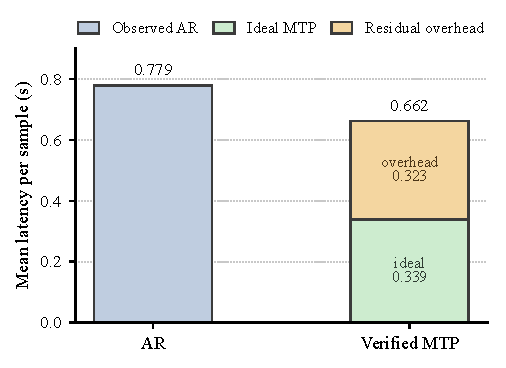
\includegraphics[width=\columnwidth]{mtp_latency_accounting.pdf}
\caption{Latency accounting for Qwen AR and verified MTP on WikiLingua.
The ideal component divides AR latency by emitted tokens per step.
Residual is the remaining latency.}
\label{fig:mtp-latency}
\end{figure}

For the Qwen WikiLingua system, verified MTP improves real throughput.
The resulting speedup remains modest.
MTP speed still depends on implementation details.

\subsection{Comparison with End-to-End Context Compression}

The comparison with LCLMs is conceptual rather than empirical, since the current project does not include an LCLM baseline.
As summarized in Table~\ref{tab:lclm-position}, LCLMs compress contexts into shorter latent sequences for general long-context inference \citep{li2026contextcompression}.
LLM2Seq keeps token-level source memory and trains for Vietnamese summarization.
The distinction matters because LLM2Seq does not optimize compression ratio; it studies whether token-level LLM states can work as source memory for summarization.
A fair future comparison should add block compression baselines, such as mean-pooling encoder states by 4, 8, or 16 tokens before the decoder.

\subsection{Qualitative Example}

Appendix~\ref{app:qualitative} gives examples from the WikiLingua test prediction files.
It shows the same pattern as the aggregate results.
LLM2Seq-Llama is short but loses key content.
LLM2Seq-Qwen often keeps the broad topic and a concise style, but it can also make serious semantic errors.
T5Gemma is more fluent and covers more details, but it is also longer.
The WikiLingua example matches the table.
Different LLM2Seq configurations choose different content and output lengths.

\subsection{Error Analysis}

The WikiLingua results reveal three error patterns.
First, on WikiLingua, LLM2Seq-Llama under-generates, which hurts recall and leads to lower ROUGE.
Second, on WikiLingua, T5Gemma often generates much longer summaries.
Longer outputs can improve overlap scores but reduce conciseness.
Third, on WikiLingua, verified MTP improves throughput only modestly.
It emits multiple tokens per step, but the verifier still costs time.

\section{System Demonstration}
\label{sec:demo}

We implement a web interface for running LLM2Seq summarization.
The interface loads the Qwen-based model, accepts a source document, and shows the generated summary.
It supports two modes.
Autoregressive mode generates one token at a time.
Verified MTP mode drafts future tokens and verifies them with the frozen decoder.
The demo reports latency, generated tokens, tokens per second, and accepted-token statistics.
Appendix~\ref{app:demo} shows the interface.
The demo is intended for qualitative inspection, while the main evidence comes from the evaluation logs.

\section{Discussion}
\label{sec:discussion}

LLM2Seq shows that LLM-based encoders can be reused inside an encoder-decoder summarizer.
On WikiLingua, the Qwen variant improves substantially over the Llama configuration while producing shorter summaries than T5Gemma, but it remains behind T5Gemma on all three ROUGE metrics.
The comparison between Qwen and Llama should be interpreted as a system-level comparison, since changing the encoder also changes the tokenizer, vocabulary, and representation space.
For Qwen on WikiLingua, MTP gives 2.30 tokens per step but only 1.17x real speedup, so accepted tokens help only when they compensate for verification overhead.
Token-level memory is useful when the summary needs local source evidence, which differs from fixed-ratio context compression \citep{li2026contextcompression}.
The current verified decoder is an implementation-level prototype.
Future deployment should fuse verification, reduce Python control flow, and use optimized runtimes such as vLLM.
Quantization methods such as SmoothQuant may also help under memory limits \citep{xiao2023smoothquant}.

\section{Threats to Validity}
\label{sec:validity}

There are five main threats.
First, the quality evaluation covers two Vietnamese summarization datasets: WikiLingua \citep{ladhak2020wikilingua} and LR-Sum \citep{palen-michel-lignos-2023-lr}.
Even so, both are written-document summarization datasets.
The result may not transfer to dialogue, legal text, scientific text, or other domains.
Second, the report uses T5Gemma as the main baseline.
It does not include many other baselines such as mT5, viT5, mBART, or prompted LLMs.
Third, Llama and Qwen differ in tokenizer, vocabulary, and representation space.
So their comparison is not a pure encoder-only ablation.
Fourth, ROUGE and BERTScore do not fully measure factuality or usefulness.
They should be read with qualitative examples.
Fifth, the WikiLingua MTP speed result depends on the current implementation.
Verifier cost, cache handling, and Python control flow can reduce speedup.

\section{Conclusion}
\label{sec:conclusion}

LLM2Seq studies how to build an encoder-decoder summarizer from repurposed LLM-based encoders.
The model uses a gated residual adapter to map source-side LLM states into decoder memory.
It then uses a lightweight cross-attentive decoder to generate summaries.
On Vietnamese WikiLingua, the Qwen-based variant improves over the Llama configuration and produces shorter summaries, but it remains behind T5Gemma on ROUGE.
On Vietnamese LR-Sum, LLM2Seq-Qwen improves over LLM2Seq-Llama but still trails T5Gemma.
Self-distilled MTP gives a real 1.17x speedup for Qwen on WikiLingua.
Future work should add adapter ablations, add compression baselines, and optimize verified decoding.

\section*{Limitations}

This report does not include a full adapter ablation.
It cannot isolate the contribution of layer fusion, salience gating, EncStack refinement, or global memory tokens.
It also does not include an LCLM-style block-compression baseline.
The comparison with context compression is therefore conceptual.
The evaluation relies on automatic metrics and does not include human factuality judgments.
Finally, the current demo is an engineering artifact for inspection, not evidence for user-facing reliability.

\section*{Ethics Statement}

This work uses an existing public summarization dataset and does not introduce human-subject data collection.
The system may still produce incomplete or incorrect summaries.
It should not be used as the only source of information in high-stakes settings.

\section*{Broader Impact}

LLM2Seq may make summarization systems easier to build from existing LLM checkpoints.
This can reduce training cost and make summarization more accessible for lower-resource languages.
At the same time, better summarization tools can also spread errors faster if users over-trust generated summaries.

\section*{Code Availability}

The repository includes the implementation, evaluation scripts, verified MTP decoding code, and the demo interface:
\href{https://github.com/BienKieu1411/LLM2Seq}{\texttt{github.com/BienKieu1411/LLM2Seq}}.

\section*{Acknowledgments}

We thank the project reviewers for feedback on framing, experimental reporting, and report structure.

\bibliography{custom}

\appendix

\section{Summary of Hyperparameters}
\label{app:hparams}

The main hyperparameters are:
\begin{itemize}
    \item Source and target length: 3,072 source tokens for both datasets; 384 target tokens for WikiLingua; 256 target tokens for LR-Sum.
    \item Generation: greedy decoding; at most 256 new tokens; no-repeat trigram blocking.
    \item Adapter: selected layers $[-1,-4,-8,-12]$; salience gate; 4-layer EncStack; 16 global memory tokens.
    \item Decoder: 8 layers; hidden size 1024; 16 heads; FFN size 4096; dropout 0.1.
    \item LoRA: encoder adapters are used during Phase 2.
    \item WikiLingua MTP: 4 heads; CE weight 0.6; KL weight 0.2; head weights $[1.0,0.8,0.5,0.25]$.
\end{itemize}

\section{Additional Experimental Results}

The current project snapshot includes the main quality and length results, plus the WikiLingua speed and MTP results reported in this report.
It does not include a complete adapter ablation.
For that reason, this report does not include an ablation table.

\section{Additional Qualitative Examples}
\label{app:qualitative}

\subsection{Representative Case}

The following example comes from test item \texttt{test\_001852}.
The source is a Vietnamese WikiHow-style article about treating hidden pimples.
We show a source excerpt for space.

\paragraph{Source (excerpt).}
Tùy vào loại da và mức độ nghiêm trọng của mụn ẩn mà bạn nên cân nhắc giữa phương pháp chườm ấm với chườm lạnh (chườm đá viên).
Chườm ấm có thể giúp làm khô mụn ẩn và dẫn lưu mụn; trong khi đó, chườm lạnh giúp giảm sưng đau tại vị trí mụn.
Không nên chườm đá trong giai đoạn đầu của mụn ẩn.
Nếu là mụn lớn, viêm nghiêm trọng hơn hoặc đau hơn, bạn nên chườm ấm để rút dịch trong mụn ra.
Bạn có thể tạo miếng chườm ấm đơn giản bằng cách nhúng khăn sạch vào nước ấm hoặc nước nóng.

\paragraph{Reference.}
Chườm ấm hoặc chườm lạnh.
Làm mặt nạ táo và mật ong.
Dùng tinh dầu tràm trà.
Thoa lô hội.

\paragraph{LLM2Seq-Llama.}
Dùng gel lô hội.
Thoa sữa rửa mặt nhẹ dịu.
Dù bằng dầu tràm trà.
Dưỡng ẩm cho da.

\paragraph{LLM2Seq-Qwen.}
Chườm đá viên lên mụn.
Chườm gạc ấm lên mụn để giảm đau và giảm đau.
Sử dụng tinh dầu tràm trà để giảm viêm và giảm chất lỏng.
Sử hưởng dầu hạt lô hội để xử lý các vấn đề của mụn có thể làm giảm mụn trứng cá.

\paragraph{T5Gemma.}
Chườm ấm hoặc chườm lạnh.
Thử dùng táo và mật ong để điều trị mụn ẩn.
Dùng tinh dầu tràm trà nếu bạn không có các phương pháp khác.
Sử dụng lô hội (nha đam) cho hiệu quả tốt nhất, nhưng hãy cẩn thận với những tác động phụ của nó khi sử dụng thường xuyên.

\paragraph{Comment.}
The three systems recover some topical-treatment actions.
LLM2Seq-Llama is short and misses the warm/cold compress step.
LLM2Seq-Qwen covers the compress and tea-tree oil ideas, but it repeats phrases and contains awkward wording.
T5Gemma is more complete and fluent, but also longer.

\subsection{Failure Case}

The following example comes from test item \texttt{test\_002672}.
The source is a Vietnamese WikiHow-style article about crying and emotional expression.
We show a source excerpt for space.

\paragraph{Source (excerpt).}
Bạn đã được dạy rằng những người dũng cảm thì thường không khóc?
Những người được dạy cách kiềm chế và giấu kín cảm xúc từ bé thường gặp khó khăn trong việc biểu lộ cảm xúc khi họ lớn lên.
Nhưng khóc là một phần thiết yếu của cuộc sống giúp cải thiện tâm lý.
Khóc có thể là biểu hiện của nỗi buồn, sự đau đớn, nỗi sợ, hạnh phúc, hay thậm chí là niềm vui.

\paragraph{Reference.}
Quên hết những gì đã biết về khóc.
Hiểu được lợi ích của khóc.
Tìm hiểu lý do tại sao bạn phải kiềm chế cảm xúc.
Cho phép chính mình khóc cũng là một cách chăm sóc bản thân tốt hơn.

\paragraph{LLM2Seq-Llama.}
Nhận biết cảm giác tội lỗi và hành động.
Xác định những suy nghĩ tiêu cực trong cuộc sống của bạn.
Tìm kiếm sự trợ giúp chuyên nghiệp.

\paragraph{LLM2Seq-Qwen.}
Hãy hiểu rằng cảm xúc của bạn là bình thường.
Hãy làm gì đó.
Hãy để bản thân bị trầm cảm.
Hãy cho phép bản thân cảm nhận sự khóc.
Hãy nhớ rằng việc phải là người luôn bộc lộ bản thân.
Hãy cười ra khỏi vùng an toàn của bạn.
Hãy vui vẻ và đau khổ.

\paragraph{T5Gemma.}
Khóc là một cách tự nhiên để thể hiện cảm xúc.
Khóc không chỉ dành riêng cho trẻ em, mà còn có ích lợi đối với người lớn tuổi như bạn.
Cố gắng khóc khi cần thiết và đừng ngại ngùng nếu mình đã bắt đầu rơi nước mắt.
Hãy nhớ rằng việc biểu lộ những cảm xúc của bản thân sẽ giúp cải thiện tâm trạng.
Thử tưởng tượng về thời điểm trước đây khi bạn bật khóc vì điều gì đó.

\paragraph{Comment.}
This example shows that LLM2Seq-Qwen can preserve conciseness but may produce wrong or unnatural phrases.
This motivates future factuality and human evaluation.
It also shows why automatic overlap and length statistics must be read together with output inspection.

\section{Demo Interface Details}
\label{app:demo}

The demo provides a source text box, a decoding-mode selector, and a maximum-token control.
It reports the generated summary, latency, generated tokens, and tokens per second.
In verified MTP mode it additionally reports accepted-token statistics.

\begin{figure*}[t]
\centering
\begin{minipage}{0.49\textwidth}
\centering
\framedemoimage{figures/demo_autoregressive_cropped.pdf}
\end{minipage}
\hfill
\begin{minipage}{0.49\textwidth}
\centering
\framedemoimage{figures/demo_mtp_cropped.pdf}
\end{minipage}
\caption{LLM2Seq web demo on the same WikiLingua sample. Left: standard autoregressive decoding. Right: verified MTP decoding.}
\label{fig:demo}
\end{figure*}

\section{Architecture Details}

The adapter uses token-wise layer fusion, a gated residual projection, token salience gating, EncStack memory refinement, and learned global memory tokens.
The EncStack directly applies standard Transformer encoder refinement.
Layer fusion, token salience gating, and learned global memory tokens adapt common conditioning ideas.
These include contextual layer mixing, feature modulation, and continuous prompt tokens.
The decoder attends to the final memory $M$ through cross-attention in every layer.

\end{document}
